
\let\negmedspace\undefined
\let\negthickspace\undefined
\documentclass[journal,12pt,twocolumn]{IEEEtran}
\usepackage{cite}
\usepackage{amsmath,amssymb,amsfonts,amsthm}
\usepackage{algorithmic}
\usepackage{graphicx}
\usepackage{textcomp}
\usepackage{xcolor}
\usepackage{txfonts}
\usepackage{listings}
\usepackage{enumitem}
\usepackage{mathtools}
\usepackage{gensymb}
\usepackage[breaklinks=true]{hyperref}
\usepackage{tkz-euclide} % loads  TikZ and tkz-base
\usepackage{listings}

\DeclareMathOperator*{\Res}{Res}
%\renewcommand{\baselinestretch}{2}
\renewcommand\thesection{\arabic{section}}
\renewcommand\thesubsection{\thesection.\arabic{subsection}}
\renewcommand\thesubsubsection{\thesubsection.\arabic{subsubsection}}

\renewcommand\thesectiondis{\arabic{section}}
\renewcommand\thesubsectiondis{\thesectiondis.\arabic{subsection}}
\renewcommand\thesubsubsectiondis{\thesubsectiondis.\arabic{subsubsection}}

% correct bad hyphenation here
\hyphenation{op-tical net-works semi-conduc-tor}
\def\inputGnumericTable{}                                 %%

\lstset{
%language=C,
frame=single, 
breaklines=true,
columns=fullflexible
}
%\lstset{
%language=tex,
%frame=single, 
%breaklines=true
%}

\begin{document}
%


\newtheorem{theorem}{Theorem}[section]
\newtheorem{problem}{Problem}
\newtheorem{proposition}{Proposition}[section]
\newtheorem{lemma}{Lemma}[section]
\newtheorem{corollary}[theorem]{Corollary}
\newtheorem{example}{Example}[section]
\newtheorem{definition}[problem]{Definition}
%\newtheorem{thm}{Theorem}[section] 
%\newtheorem{defn}[thm]{Definition}
%\newtheorem{algorithm}{Algorithm}[section]
%\newtheorem{cor}{Corollary}
\newcommand{\BEQA}{\begin{eqnarray}}
\newcommand{\EEQA}{\end{eqnarray}}
\newcommand{\define}{\stackrel{\triangle}{=}}

\bibliographystyle{IEEEtran}
%\bibliographystyle{ieeetr}


\providecommand{\mbf}{\mathbf}
\providecommand{\pr}[1]{\ensuremath{\Pr\left(#1\right)}}
\providecommand{\qfunc}[1]{\ensuremath{Q\left(#1\right)}}
\providecommand{\sbrak}[1]{\ensuremath{{}\left[#1\right]}}
\providecommand{\lsbrak}[1]{\ensuremath{{}\left[#1\right.}}
\providecommand{\rsbrak}[1]{\ensuremath{{}\left.#1\right]}}
\providecommand{\brak}[1]{\ensuremath{\left(#1\right)}}
\providecommand{\lbrak}[1]{\ensuremath{\left(#1\right.}}
\providecommand{\rbrak}[1]{\ensuremath{\left.#1\right)}}
\providecommand{\cbrak}[1]{\ensuremath{\left\{#1\right\}}}
\providecommand{\lcbrak}[1]{\ensuremath{\left\{#1\right.}}
\providecommand{\rcbrak}[1]{\ensuremath{\left.#1\right\}}}
\theoremstyle{remark}
\newtheorem{rem}{Remark}
\newcommand{\sgn}{\mathop{\mathrm{sgn}}}
\providecommand{\abs}[1]{\left\vert#1\right\vert}
\providecommand{\res}[1]{\Res\displaylimits_{#1}} 
\providecommand{\norm}[1]{\left\lVert#1\right\rVert}
%\providecommand{\norm}[1]{\lVert#1\rVert}
\providecommand{\mtx}[1]{\mathbf{#1}}
\providecommand{\mean}[1]{E\left[ #1 \right]}
\providecommand{\fourier}{\overset{\mathcal{F}}{ \rightleftharpoons}}
%\providecommand{\hilbert}{\overset{\mathcal{H}}{ \rightleftharpoons}}
\providecommand{\system}{\overset{\mathcal{H}}{ \longleftrightarrow}}
	%\newcommand{\solution}[2]{\textbf{Solution:}{#1}}
\newcommand{\solution}{\noindent \textbf{Solution: }}
\newcommand{\cosec}{\,\text{cosec}\,}
\providecommand{\dec}[2]{\ensuremath{\overset{#1}{\underset{#2}{\gtrless}}}}
\newcommand{\myvec}[1]{\ensuremath{\begin{pmatrix}#1\end{pmatrix}}}
\newcommand{\mydet}[1]{\ensuremath{\begin{vmatrix}#1\end{vmatrix}}}

\let\vec\mathbf

\vspace{3cm}

\title{
\textbf{Assignment 1} \\ \large \textbf{AI1110}: Probability and Random Variables 


}
\author{ Rishitha Surineni\\ cs22btech11050} 
	



% make the title area
\maketitle

\newpage

%\tableofcontents

\bigskip

\renewcommand{\thefigure}{\theenumi}
\renewcommand{\thetable}{\theenumi}

\textbf{12.13.1.15: Question:}\\
 	Consider the experiment of throwing a die,if a multiple of 3 comes up,throw the die again and if any other number comes,toss a coin.Repeat this experiment till a coin is tossed.Find the conditional probability of the event `the coin shows a tail',given that `at least one die shows a 3'.
 \\\textbf{Answer:$\frac{1}{2}$.}
 \\\textbf{Solution:}
 \\
 The given experiment is a Markov Process and the following is the Markov Chain Diagram for this experiment.
 \begin{figure}[h]
\centering
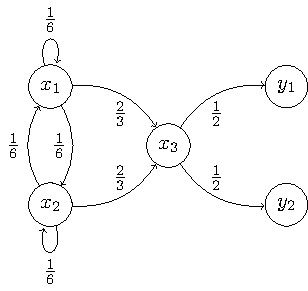
\includegraphics[width=\columnwidth]{./Figure/figure.pdf}
\caption { Markov Chain Diagram }
\end{figure}
\\The states in the Diagram are defined as follows,
\\State $x_1$ : Die roll results in 3 and the die is to be rolled again.
\\State $x_2$ : Die roll results in 6 and the die is to be rolled again.
\\State $x_3$ : Die roll results in not a multiple of 3 and a coin is to be tossed now.
\\State $y_1$ : Coin toss results in Tail
\\State $y_2$ : Coin toss results in Head
\\ Need to Find, Conditional Probability of the event `the coin shows a tail',given that `at least one die shows a 3', i.e., $\pr{y_1|x_1,x_3} $
\\$\pr{y_1|x_1,x_3}$ refers to Conditional Probability of being in state $y_1$ given that the Markov chain has been in state $x_1$ atleast once and has also visited state $x_3$.
\begin{align}
       \pr{y_1|x_1,x_3} = \frac{\pr{y_1,x_3|x_1}}{\pr{x_3|x_1}}
    \end{align}
$\pr{y_1,x_3|x_1}$ refers to the Probability that Markov Chain transitions from state $x_1$ to state $x_3$ and then to state $y_1$.
\\This Markov Chain is time homogenous . So,
\begin{align}
        \pr{y_1,x_3|x_1} &= \pr{y_1|x_3}\pr{x_3|x_1}\\
        \pr{y_1|x_1,x_3} &=\frac{\pr{y_1|x_3}\pr{x_3|x_1}}{\pr{x_3|x_1}}\\
        \pr{y_1|x_1,x_3} &= \pr{y_1|x_3}\\
        \pr{y_1|x_1,x_3} &= \frac{1}{2}
    \end{align}
Hence,
\\Probability of the event `the coin shows a tail',given that `at least one die shows a 3' is $\frac{1}{2}$.
\end {document}